% !TEX root = ./AM_2C-Testes_Resolucoes-2022.1.2.tex
\providecommand\mainfilename{"./AM_2C-Testes_Resolucoes.tex"}
\providecommand \subfilename{}
\renewcommand   \subfilename{"./AM_2C-Testes_Resolucoes-2022.1.2.tex"}
\documentclass[\mainfilename]{subfiles}

% \graphicspath{{\subfix{../images/}}}
% \tikzset{external/force remake=true}

\begin{document}

\mymakesubfile{2}
{AM\,2C -- Teste 2 2022.1 Resolução}
{AM\,2C -- Teste 2 2022.1 Resolução}

\group{}

\begin{questionBox}1{}
    
    Considere o 

    \begin{BM}
        \int_0^1
        \left(
            \int_y^1
            x^2\,e^{x\,y}
            \,\odif{x}
        \right)
        \odif{y}
    \end{BM}

    Tambem pode ser escrito:

    \begin{flalign*}
        &
            \left.
                \begin{aligned}
                    x = 1;
                 \\ x = y;
                 \\ y = 0;
                 \\ y = 1;
                \end{aligned}
            \right\}
            \implies &\\&
            \implies
            \int_0^1
            \left(
                \int_x^1
                x^2\,e^{x\,y}
                \,\odif{y}
            \right)
            \odif{x}
            = \int_0^1
            \left(
                x^2
                \left. 
                    \Delta e^{x\,y}/x 
                \right\rvert_x^1
            \right)
            \odif{x}
            = \int_0^1
            \left(
                x
                \left(
                    e^{x} - e^{x^2}
                \right)
            \right)
            \odif{x}
            = &\\&
            = \frac{e-1}{x}
        &
    \end{flalign*}
    
\end{questionBox}






\begin{questionBox}1m{}
    
    \begin{BM}
        \mathcal{E}sfera: x^2+y^2+z^2=1
     \\ z= 1/3
     \\ z= 1/2
    \end{BM}

    integral de coordenadas polares

    \begin{flalign*}
        &
            x^2 + y^2 + (1/3)^2 = 1
            \implies
            x^2 + y^2 = 8/9
            \implies
            \rho_1 
            = \tan^{-1} \sqrt{8/9}/(1/3)
        &\\[2ex]&
             x^2 + y^2 + (1/2)^2 = 1
            \implies
            x^2 + y^2 = 1/2
            \implies
            \rho_2 
            = \sqrt{(1/2)^2 + 1/2}
            = \sqrt{3}/2
            % \int
            % \left(
            %     \int_0
            %     \frac
            %         {1\lor\rho}
            %         {\sqrt{1\pm\rho^2}}
            %     \,\odif{\rho}
            % \right)
            % \odif{\theta}
            &\\[3ex]&
            \implies
            \int
            \left(
                \int
                \frac
                    {1\lor\rho}
                    {\sqrt{1\pm\rho^2}}
                \,\odif{\rho}
            \right)
            \odif{\theta}
        &
    \end{flalign*}
    
\end{questionBox}

\begin{questionBox}1{}
    
    A função potencial \(\varphi(x,y,z)\) do campo conservativo

    \begin{BM}
        \vec{u}
        = \left\{
            \begin{aligned}
               &\left(
                    \frac{y}{x^2}
                    - \frac{1}{z}
                    + y^2\,z\,e^{x\,y^2\,z}
                \right)\,\hat{\imath}
             \\&+ \left(
                    - \frac{1}{x}
                    + 2\,x\,y\,z\,e^{x\,y^2\,z}
                    - 2
                \right)\,\hat{\jmath}
             \\&+ \left(
                    \frac{x}{z^2}
                    + x\,y^2\,e^{x\,y^2\,z}
                    - 2\,z
                \right)\,\hat{k}
            \end{aligned}
        \right.
        \\[2ex]
        \varphi(1,0,1) = 2
    \end{BM}

    \begin{flalign*}
        &
            \nabla\varphi(x,y,z)
            = \vec{u}
            = \left\{
                \begin{aligned}
                   &\left(
                        \frac{y}{x^2}
                        - \frac{1}{z}
                        + y^2\,z\,e^{x\,y^2\,z}
                    \right)\,\hat{\imath}
                 \\&+ \left(
                        - \frac{1}{x}
                        + 2\,x\,y\,z\,e^{x\,y^2\,z}
                        - 2
                    \right)\,\hat{\jmath}
                 \\&+ \left(
                        \frac{x}{z^2}
                        + x\,y^2\,e^{x\,y^2\,z}
                        - 2\,z
                    \right)\,\hat{k}
                \end{aligned}
            \right.
            &\\[3ex]&
            \implies
            \varphi(x,y,z)
            = \pm\frac{y}{x}
            \pm\frac{x}{z}
            + e^{x\,y^2\,z}
            + (0\lor z^2)
            + 1
        &
    \end{flalign*}
    
\end{questionBox}






\begin{questionBox}1{}
    
    As equações vetoriais do plano tangente de da reta normal à superfície de equações paramétricas
    \begin{BM}
        \left\{
        \begin{aligned}
            x &= u-v
         \\ y &= u+v
            \qquad& -2 \leq u \leq 2
         \\ z &= u^2+v^2
            \qquad& -2 \leq v \leq 2
        \end{aligned}
        \right.
    \end{BM}

    no ponto \(P_0 = (2,0,2)\) correspondente a \(u=1,v=-1\), são:

    \begin{flalign*}
        &
            &\\[3ex]&
            \implies
            \left\{
            \begin{aligned}
                T
               &= O
                + 2\,\hat{\imath}
                + 2\,\hat{k}
                + \alpha(
                    \hat{\imath}
                    \pm \hat{\jmath}
                    + 2\,\hat{k}
                )
                + \beta
                \,(
                    -\hat{\imath}
                    \pm\hat{\jmath}
                    \pm\hat{k}
                )
                \qquad& \{\alpha,\beta\}\subset\mathbb{R}
             \\ N 
               &= O
                + 2\,\hat{\imath}
                + 2\,\hat{k}
                + \lambda(
                    \pm 2\,\hat{\imath}
                    + \hat{k}
                )
                \qquad& \lambda\in\mathbb{R}
            \end{aligned}
            \right.
        &
    \end{flalign*}
    
\end{questionBox}

\begin{questionBox}1{}
    
    Seja \textit{L} a fronteira a região limitada pelas curvas de equações \(y=x^2\) e \(x=y^2\).
    O integral curvilíneo
    \begin{BM}
        \int_{L^+}
        \left(
            e^{-y}
            \odif{x}
            + y\,e^{x}\odif{y}
        \right)
    \end{BM}

    pode ser calculado a partir do integral repetido:
    
    \begin{flalign*}
        &
            \left.
                \begin{aligned}
                    y = x^2
                  \\x = y^2
                \end{aligned}
            \right\}
            \implies
        &
    \end{flalign*}

    \begin{center}
        %\pgfplotsset{height=7cm, width= .6\textwidth}
        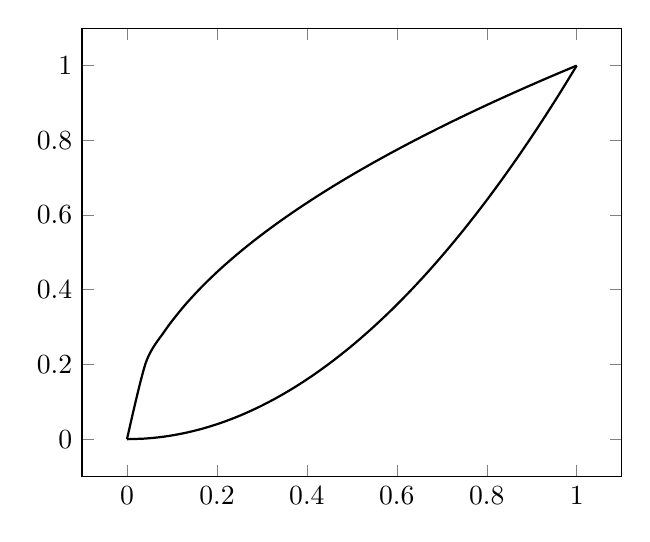
\begin{tikzpicture}
        \begin{axis}
            [
                % xmajorgrids = true,
                % legend pos  = north west
                domain   = 0:1,
                domain y = 0:1,
            ]
            % Legends
            % \addlegendimage{empty legend}
            % \addlegendentry[Red]{\( x \)}
            
            % % Plot from csv file
            % \addplot[smooth, thick, mark=*] % mesh for colormap
            % table[
            %     col sep=comma,  % csv: comma,
            %     header=true,
            %     x index=3,      % x column on file
            %     y index=4,      % y column on file
            %     point meta=x,   % value to colormap
            % ]{  file.csv };
            
            % Plot from equation
            \addplot[
                smooth,
                thick,
                % Red,
                % samples = 0.4*\mysampledensity,
            ]{  x^2 };
            % Plot from equation
            \addplot[
                smooth,
                thick,
                % Red,
                % samples = 0.4*\mysampledensity,
            ]{  sqrt(x) };
            
        \end{axis}
        \end{tikzpicture}
    \end{center}

    \begin{flalign*}
        &
            \int_{L^+}
            \left(
                e^{-y}
                \odif{x}
                + y\,e^{x}\odif{y}
            \right)
            = \int_0^1
            \left(
                \int_{\sqrt{x}}^{y^2}
                \left(
                    e^{-y}
                    \odif{x}
                    + y\,e^{x}\odif{y}
                \right)
            \right)
            \implies &\\&
            \implies
            \int_0^1
            \left(
                \int_{\sqrt{y}}^{y^2}
                \left(
                    y\,e^x
                    \pm e^{-y}
                \right)
                \odif{x}
            \right)
            \odif{y}
        &
    \end{flalign*}
    
\end{questionBox}




\newpage{}
\group{}



\begin{questionBox}1{}
    
    \begin{BM}
        \left.
            \begin{aligned}
                D: 1^\circ\text{ octante}
             \\ \limsup D: z= 2
             \\ \liminf D: x^2+y^2=z^2
             \\ \lim D: S
            \end{aligned}
        \right\}
    \end{BM}
    
    \begin{BM}
        \iint_S\left(
            \begin{aligned}
                \left(
                    x\,\sin^2(z) + e^{z^2}
                \right)\hat{\imath}
             \\ + \left(
                    y\,\cos^2(z) + e^{\cos(x)}
                \right)\hat{\jmath}
             \\ + \left(
                    2\,z + (y\,e)^y
                \right)\hat{k}
            \end{aligned}
        \right)
        \cdot\vec{n}\odif{S}
    \end{BM}

    % \begin{flalign*}
    %     &
            
    %     &
    % \end{flalign*}
    
\end{questionBox}


\newpage{}
\group{}

\begin{questionBox}1{}
    
    \begin{BM}
        S = \left\{
            (x,y,z)\in S:
            z=1-x^2-y^2
            \land
            0\leq z \leq 1
        \right\}
    \end{BM}
    
\end{questionBox}

\begin{questionBox}2{}
    
    \begin{questionBox}3{Equações Paramétricas}
        
        \begin{flalign*}
            &
                \left.
                    \begin{aligned}
                       &z=0\implies x^2+y^2 = 1
                        \implies
                        \max x = \max y = 1
                    \\&z=1\implies x^2+y^2 = 0 
                        \implies x=y=0
                    \end{aligned}
                \right\}
                \implies &\\&
                \implies
                \left\{
                    \begin{aligned}
                        x &=
                     \\ y &=
                     \\ z &=
                    \end{aligned}
                \right.
                \qquad t
            &
        \end{flalign*}
        
    \end{questionBox}

    \begin{questionBox}3{Vetor normal em qualquer ponto}
        
        
        
    \end{questionBox}
    
\end{questionBox}




\begin{questionBox}1m{}
    
    Fazendo a mudança de variáveis
    \begin{BM}
        T(u,v)
        = \left\{
            \begin{aligned}
               & x = v\,(1-u^2)
             \\& y = u
            \end{aligned}
        \right.
    \end{BM}
    Calcule
    \begin{BM}
        \iint_D
        \frac{y^2}{x}
        \odif{x,y}:\\
        D = \left\{
            (x,y,z)\in\mathbb{R}:
            \begin{aligned}
                \lim D: x=& 1-y^2
             \\ \land \lim D: x=& 3(1-y^2)
            \end{aligned}
        \right\}
    \end{BM}

    \begin{flalign*}
        &
            \left.
                \begin{aligned}
                    x = 1-y^2
                 \\ x = 3(1-y^2)
                \end{aligned}
            \right\}
            \implies
        &
    \end{flalign*}

    \begin{center}
        %\pgfplotsset{height=7cm, width= .6\textwidth}
        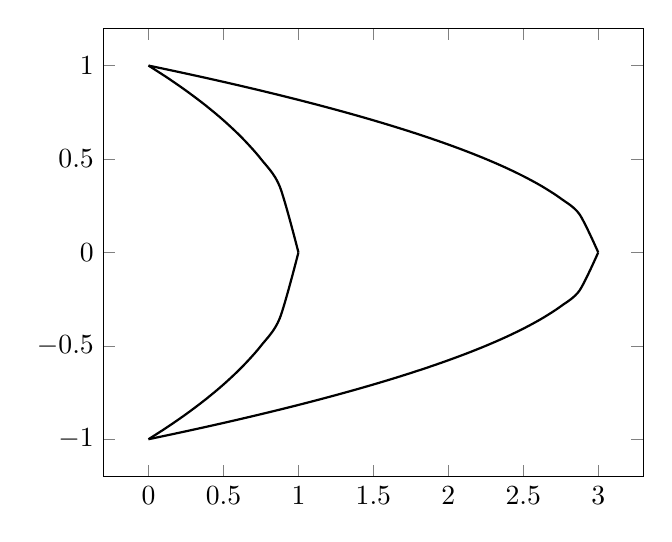
\begin{tikzpicture}
        \begin{axis}
            [
                % xmajorgrids = true,
                % legend pos  = north west
                domain = 0:3,
            ]
            % Legends
            % \addlegendimage{empty legend}
            % \addlegendentry[Red]{\( x \)}
            
            % % Plot from csv file
            % \addplot[smooth, thick, mark=*] % mesh for colormap
            % table[
            %     col sep=comma,  % csv: comma,
            %     header=true,
            %     x index=3,      % x column on file
            %     y index=4,      % y column on file
            %     point meta=x,   % value to colormap
            % ]{  file.csv };


            % Plot from equation
            \addplot[
                smooth,
                thick,
                % Red,
                % domain  = -2:2,
                % samples = 0.4*\mysampledensity,
                % variable = y
                % variable y = x
            ]{ sqrt(1-x/3) };
            \addplot[
                smooth,
                thick,
                % Red,
                % domain  = -2:2,
                % samples = 0.4*\mysampledensity,
                % variable = y
                % variable y = x
            ]{ -sqrt(1-x/3) };
            
            % Plot from equation
            \addplot[
                smooth,
                thick,
                % Red,
                % domain  = -2:2,
                % samples = 0.4*\mysampledensity,
                % variable = y
                % variable y = x
            ]{ sqrt(1-x) };
            \addplot[
                smooth,
                thick,
                % Red,
                % domain  = -2:2,
                % samples = 0.4*\mysampledensity,
                % variable = y
                % variable y = x
            ]{ -sqrt(1-x) };
            
        \end{axis}
        \end{tikzpicture}
    \end{center}

    \begin{flalign*}
        &
            \iint_D
            \frac{y^2}{x}
            \odif{x,y}
            = \int_{-1}^1
            \left(
                \int_{1-u^2}^{3(1-u^2)}
                \frac{u^2}{x}
                \odif{x}
            \right)\odif{u}
            = \int_{-1}^1
            \left(
                \int_{1-u^2}^{3(1-u^2)}
                \frac{u^2}{v(1-u^2)}
                \odv{x}{u}
                \odif{u}
            \right)\odif{u}
            = &\\&
            = \int_{-1}^1
            \left(
                \int_{1-u^2}^{3(1-u^2)}
                \frac{u^2}{v(1-u^2)}
                \odv{v(1-u^2)}{v}
                \odif{v}
            \right)\odif{u}
            = &\\&
            = \int_{-1}^1
            \left(
                \int_{1-u^2}^{3(1-u^2)}
                \frac{u^2}{v(1-u^2)}
                (1-u^2)
                \odif{v}
            \right)\odif{u}
            = \int_{-1}^1
            \left(
                \int_{1-u^2}^{3(1-u^2)}
                \frac{u^2}{v}
                \odif{v}
            \right)\odif{u}
            = &\\&
            = \int_{-1}^1
            \left(
                u^2
                \Delta\left(
                    \ln(v)
                \right)
                \rvert_{1-u^2}^{3(1-u^2)}
            \right)\odif{u}
            % = &\\&
            = \ln(3)
            \int_{-1}^1
            \left(
                u^2
            \right)\odif{u}
            = &\\&
            = \ln(3)
            \Delta\left(
                u^3/3
            \right)\rvert_{-1}^1
            = (\ln(3)/3)*0
            % = &\\&
        &
    \end{flalign*}
    
\end{questionBox}

\end{document}